\section{Methoden und Durchführung}
Zuerst soll die Kennlinie der Diode bestimmt werden. Dazu wird diese nach \cref{Aufbau} gemessen. Dabei wird die die Leistung der Mikrowellenstrahlung in Spannung umgewandelt. Dies wird auch in allen weiteren Messungen verwendet, da sich die Spannung einfacher direkt messen lässt.

%\begin{figure}[h]
%	\centering
%	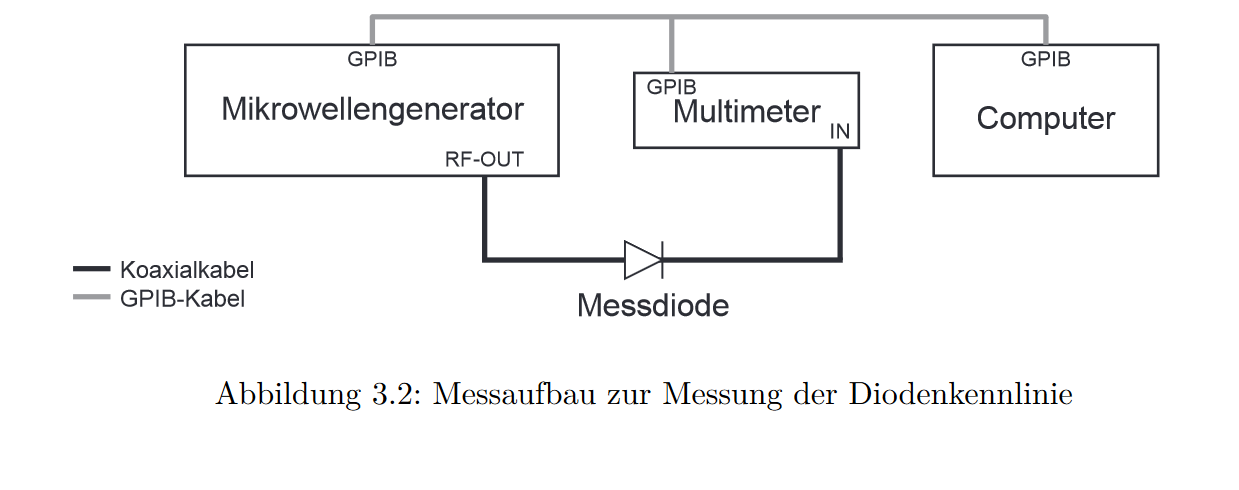
\includegraphics[scale=0.4]{../Diode_Aufbau.PNG}
%	\caption{Skizze des Versuchaufbaus}
%	\label{Aufbau}
%\end{figure}

Zuletzt sollen in zwei verschiedenen Koaxialkabeln stehende Wellen erzeugt und die Resonanzfrequenzen, bei denen die stehenden Wellen beobachtet werden, gemessen werden. Aus den Abständen zwischen den Resonanzen soll anschließend mit \cref{eq:c} die Ausbreitungsgeschwindigkeit der Welle im Kabel berechnet werden.
\begin{equation}
c = 2l(f_{n+1} - f_n)
\label{eq:c}
\end{equation}
Zuletzt soll dann mit \cref{eq:er} die relative Permittivität bestimmt werden.
\begin{equation}
\epsilon_r = \left( \frac{c_0}{c}\right) ^2
\label{eq:er}
\end{equation}

\section{Ergebnis}
\subsection{Kennlinie}
Zuerst wird die Kennlinie der Diode bestimmt. Diese wird in \cref{fuck_scidavis} dargestellt. Dabei wird mit einer e-Funktion gefittet, durch die beschrieben wird, welche Leistung in wie viel Spannung umgewandelt wird. 

\begin{figure}[h]
	\centering
	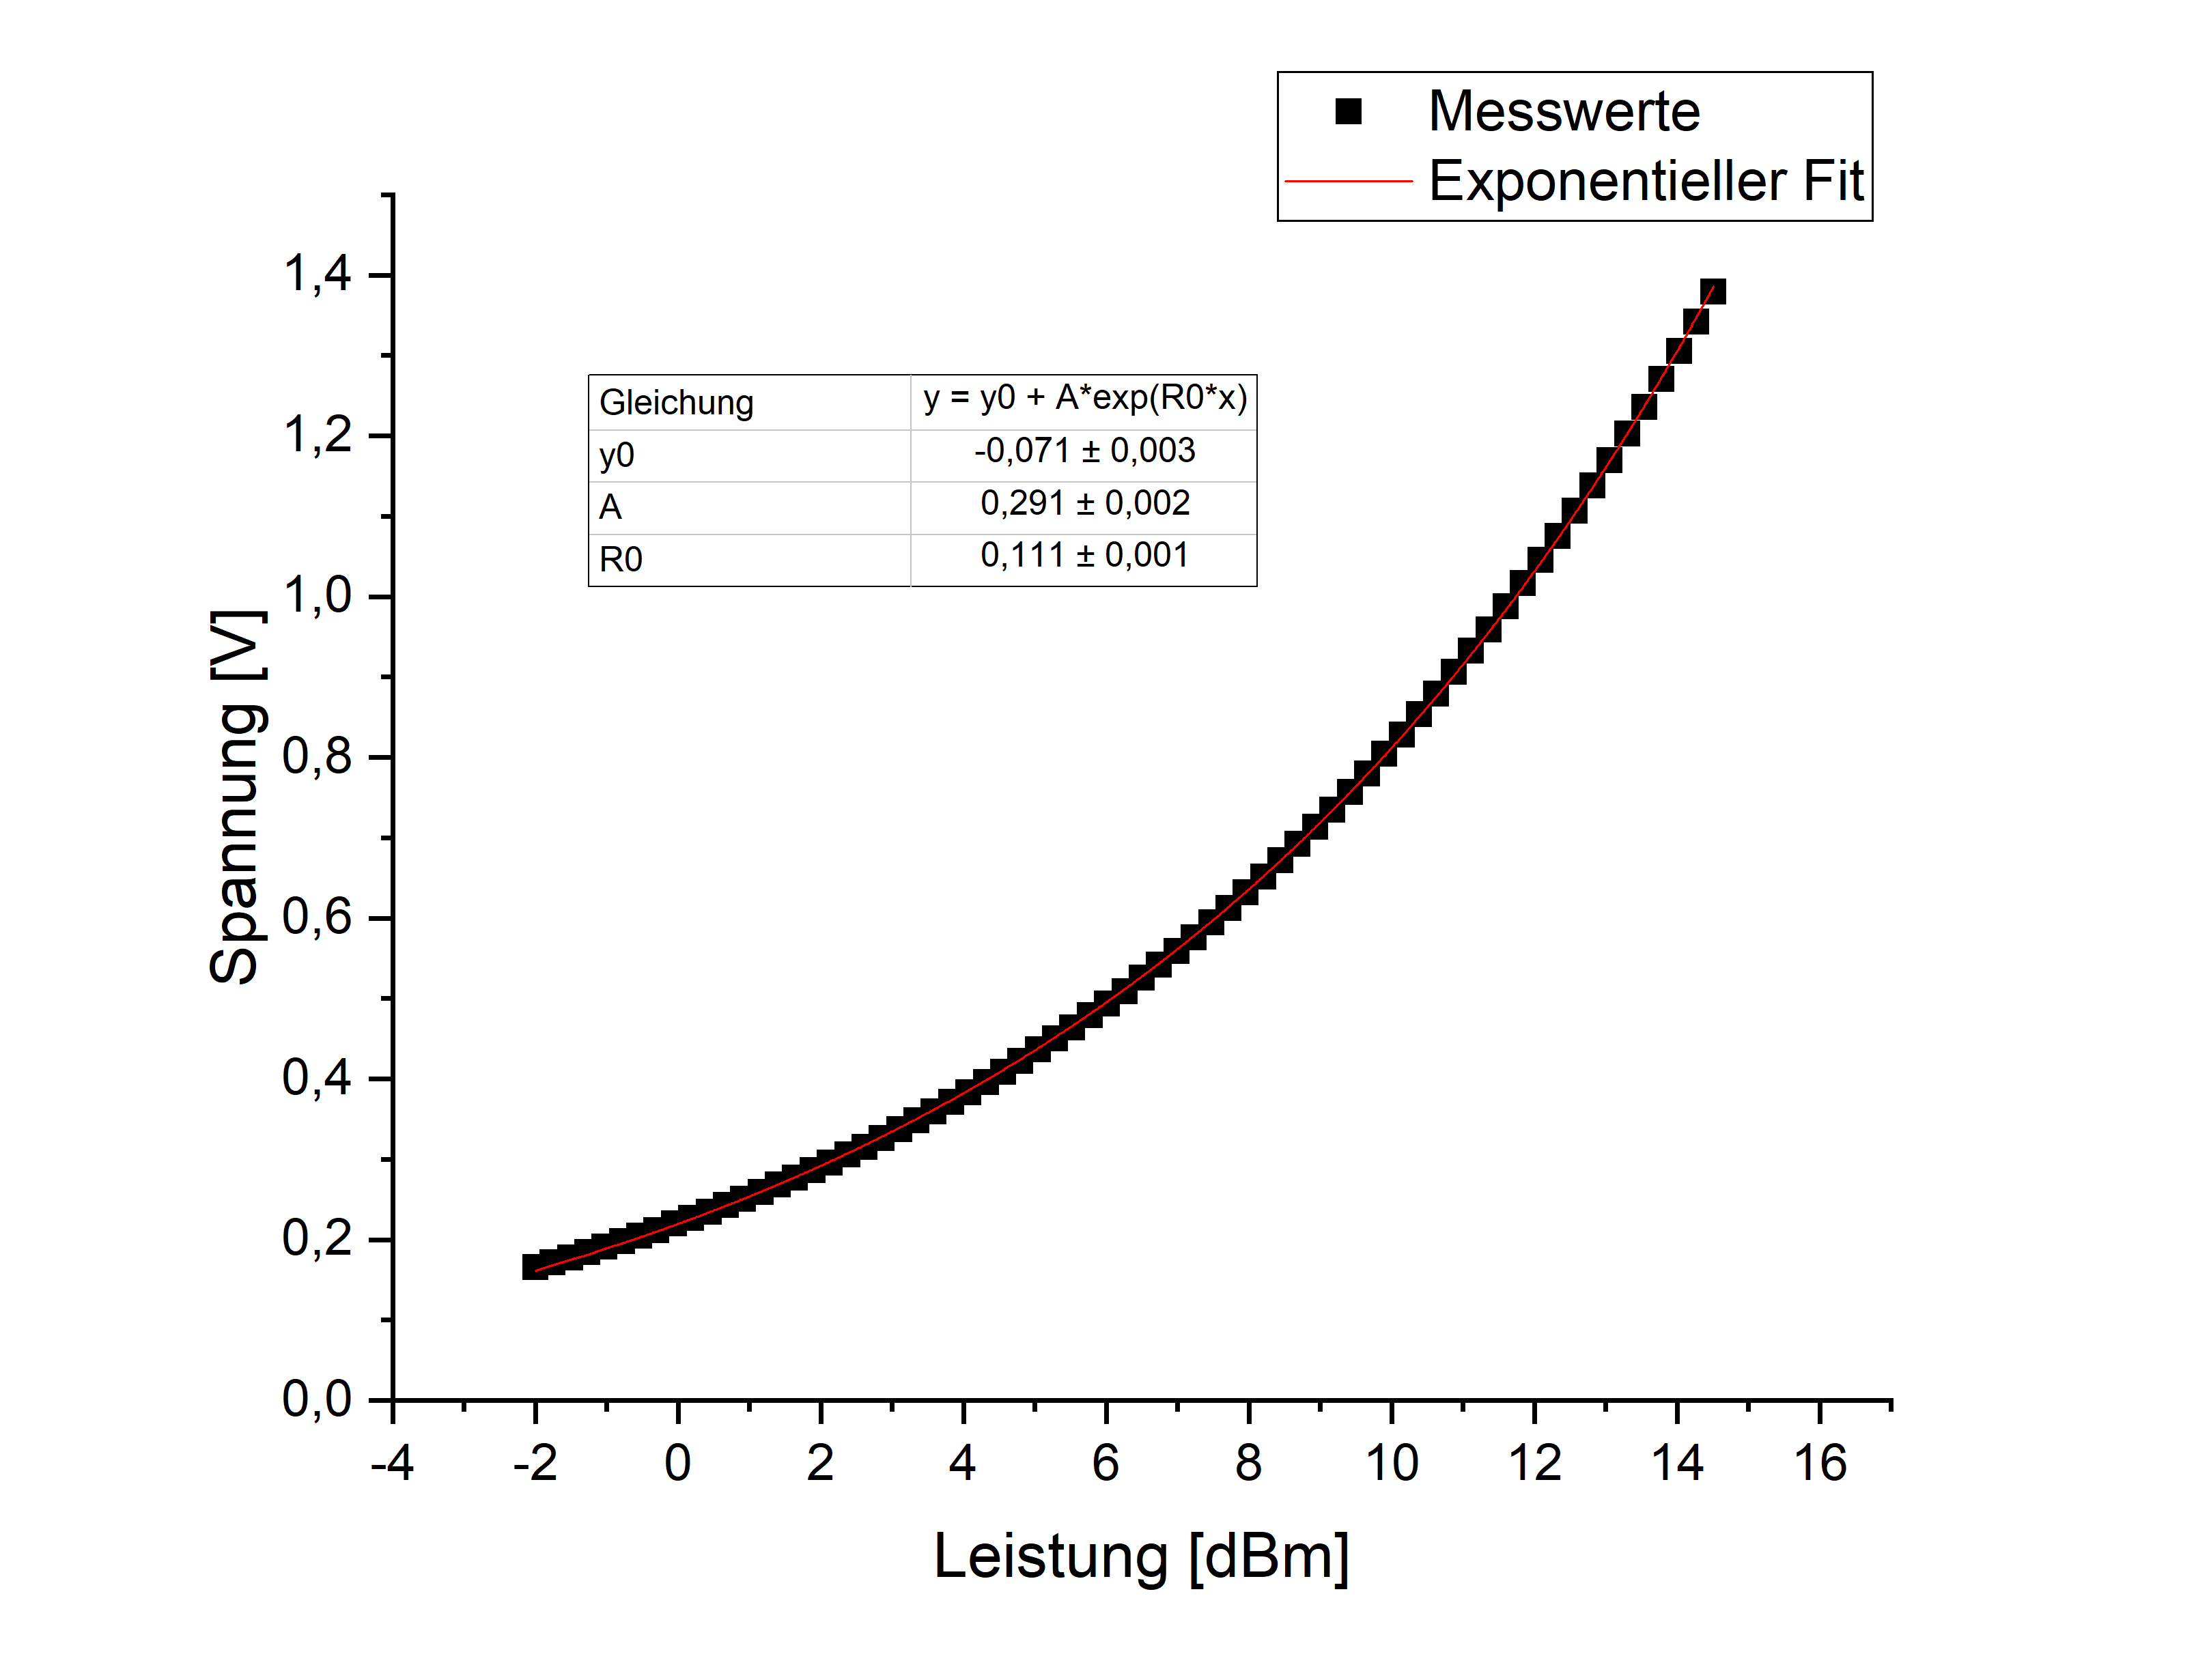
\includegraphics[scale=0.4]{fuck_scidavis.PNG}
	\caption{Kennlinie der Diode}
	\label{fuck_scidavis}
\end{figure}

\subsection{Ausbreitungsgeschwindigkeit und relative Permittivität}
Im letzten Abschnitt werden Lichtgeschwindigkeit und Permittivität zwei verschiedener Koaxialkabel bestimmt. Zuerst wurde dafür der Abstand zwischen zwei benachbarten Resonanzen bestimmt. In \cref{gleich} sind die Messergebnisse für die Messung mit Kabel 1 sowohl für offenes Kabelende als auch für kurzgeschlossenes Kabelende dargestellt. Dabei ist die Leistung in dBm gegen die Frequenz in GHz aufgetragen.

\begin{figure}[h]
	\centering
	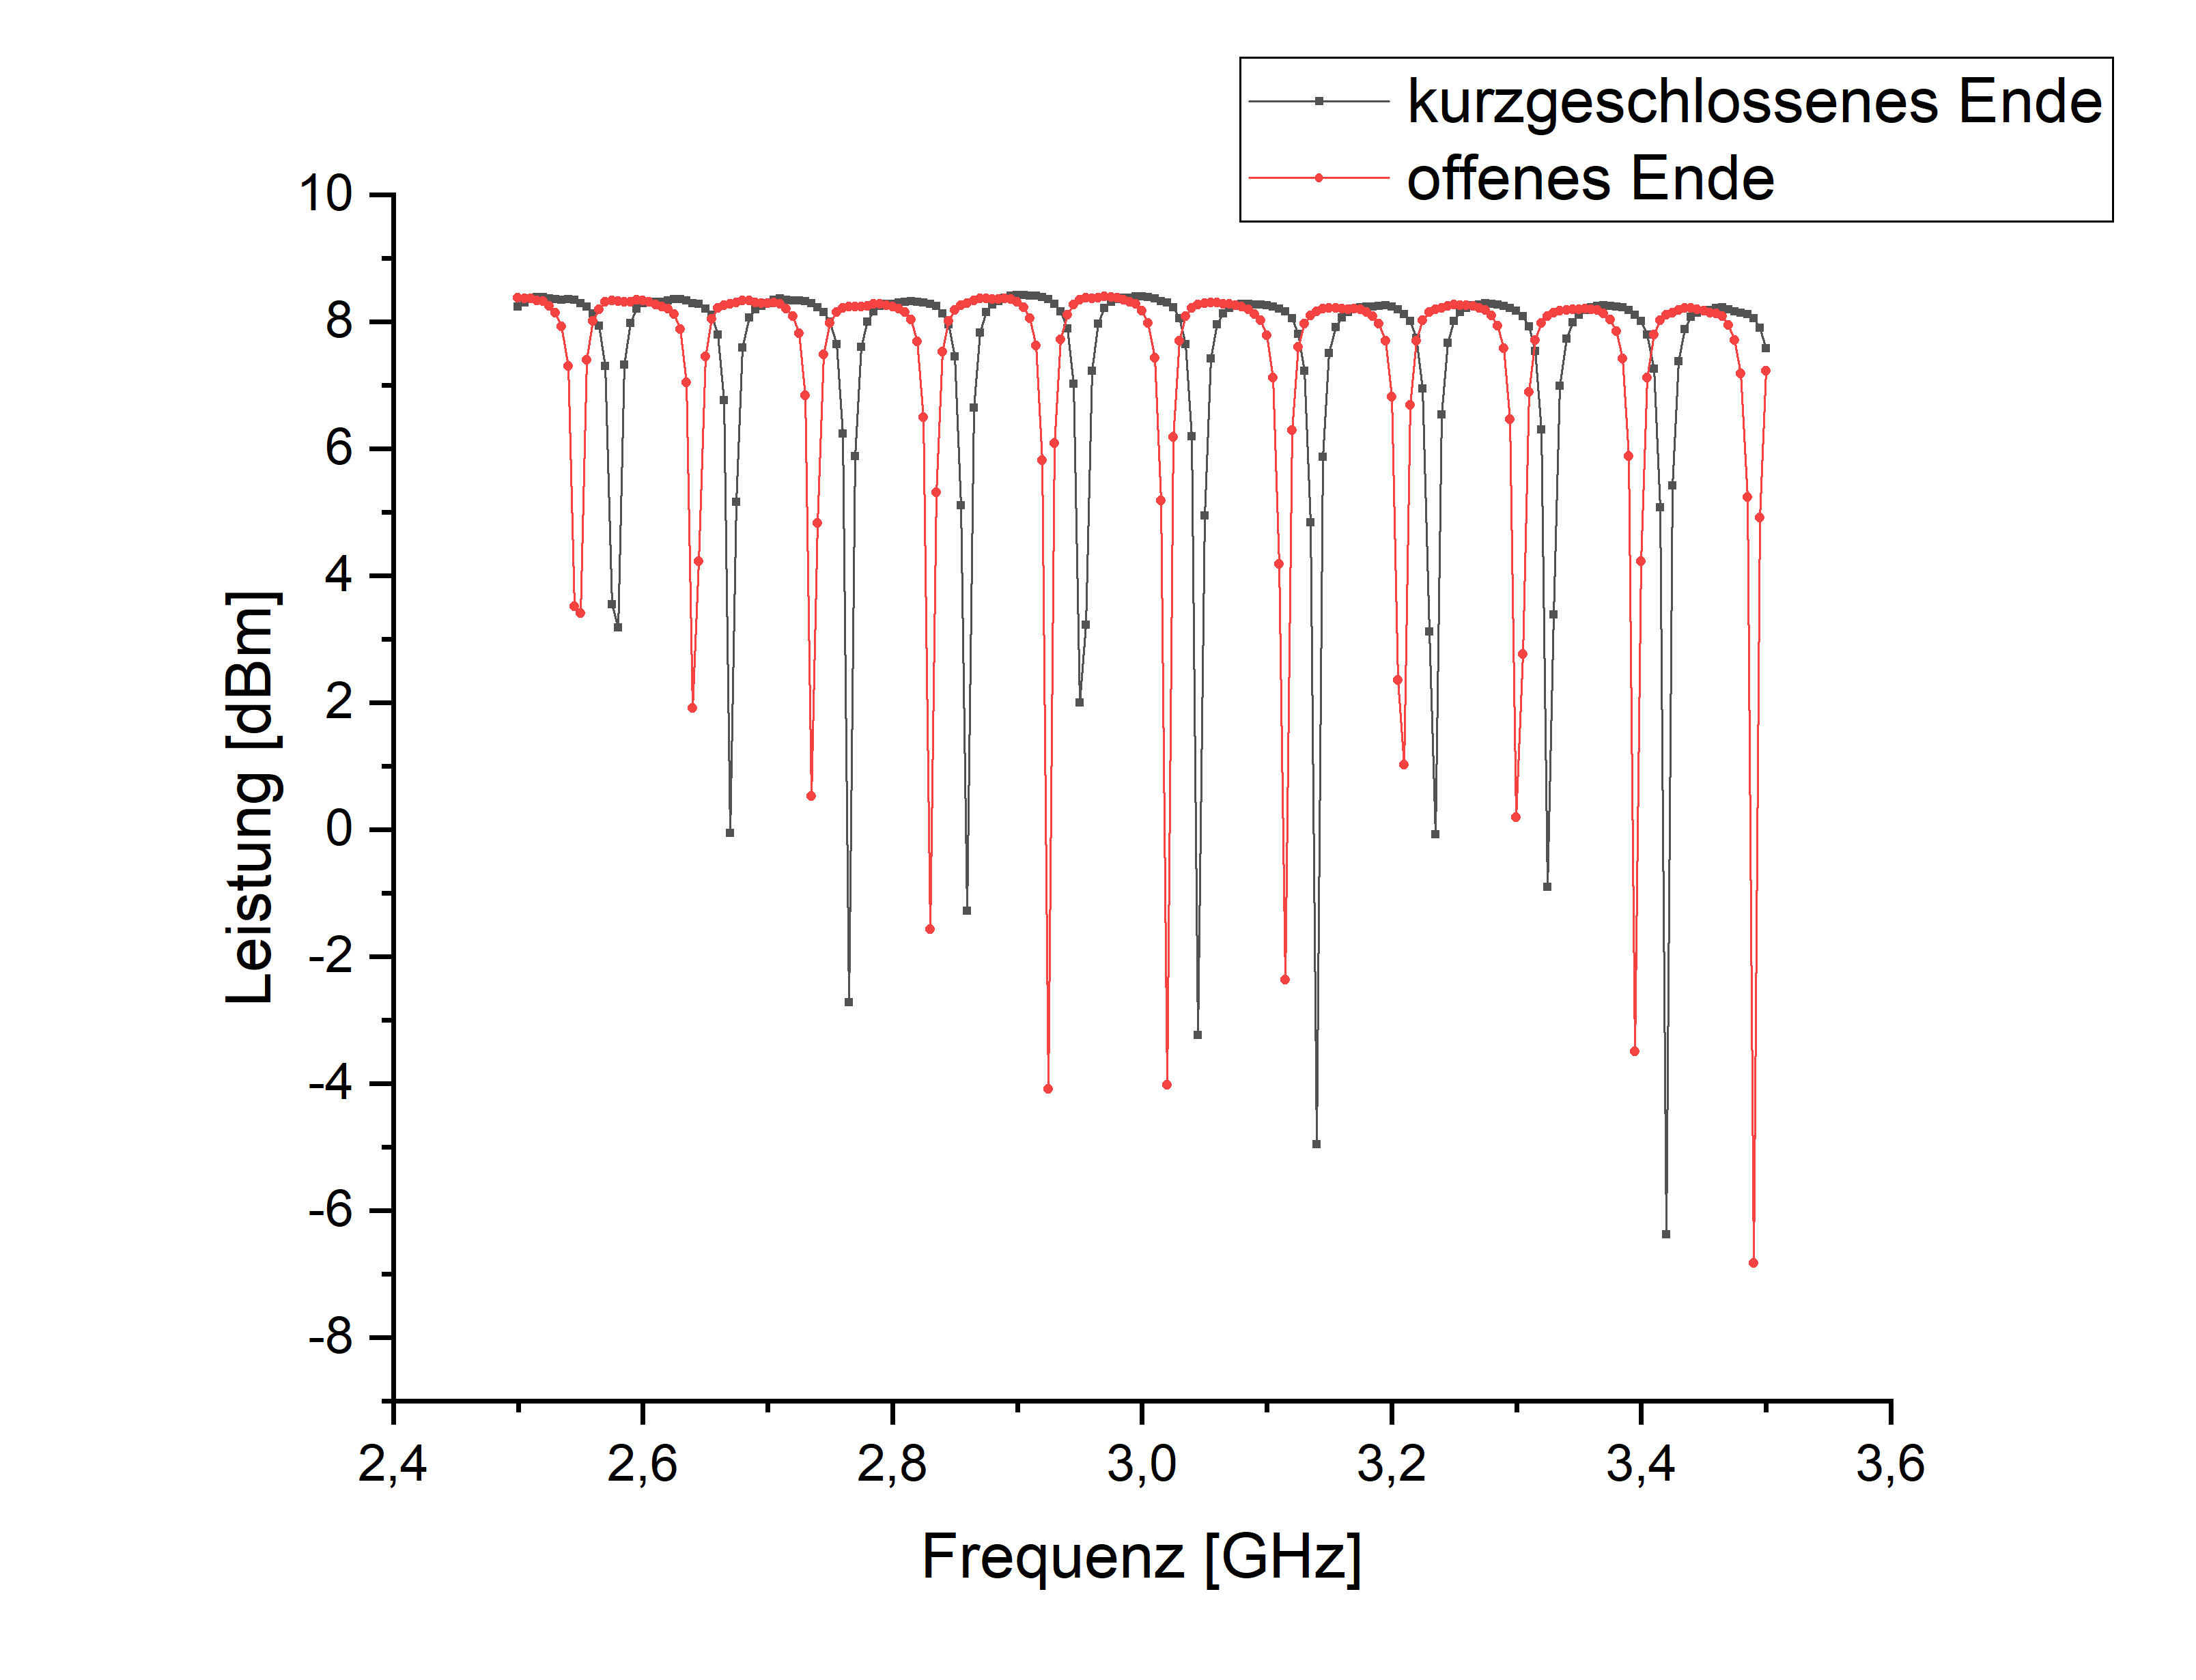
\includegraphics[scale=0.7]{gleiches_Kabel.png}
	\caption{Leistung in Abhängigkeit der Frequenz für offenes und kurzgeschlossenes Kabelende für Kabel 1. Deutlich erkennbar sind die Resonanzfrequenzen.}
	\label{gleich}
\end{figure}

Außerhalb der Resonanzen beträgt die Leistung konstant etwa $\SI{8}{dBm}$, an den Resonanzen fällt sie um mehrere Größenordnungen ab. Für beide Messungen wurde der mittlere Abstand zwischen zwei Resonanzfrequenzen ermittelt. Hierfür wurde der Mittelwert aus allen Frequenzabständen benachbarter Resonanzen gebildet. Es ergeben sich Werte von $\SI{0,094\pm0,002}{GHz}$ für das offene Kabelende und $\SI{0,093\pm0,002}{GHz}$ für das geschlossene Kabelende. Die Unsicherheit ergeben sich aus direkt aus der Standardabweichung vom Mittelwert. Die Fehler der Geräte liegen unter $0,01\%$ und können daher vernachlässigt werden. Der mittlere Abstand der beiden Resonanzfrequenzen ist im Rahmen der Unsicherheit gleich. Die Art des Abschlusswiderstands hat damit offenbar keine Auswirkung auf den Abstand der Resonanzen. Allerdings treten die Resonanzen bei kurzgeschlossenem Ende jeweils bei um etwa $\SI{300}{MHz}$ höheren Frequenzen auf als die Resonanzen bei offenem Ende.

Für ein anderes Kabel (im folgenden Kabel 2) wurde anschließend die gleiche Messung mit offenem Ende durchgeführt. In \cref{anderes} werden die Ergebnisse der Messungen mit offenem Ende beider Kabel verglichen. Direkt erkennbar ist, dass hier der Abstand zwischen zwei Resonanzen unterschiedlich ist.

\begin{figure}[h]
	\centering
	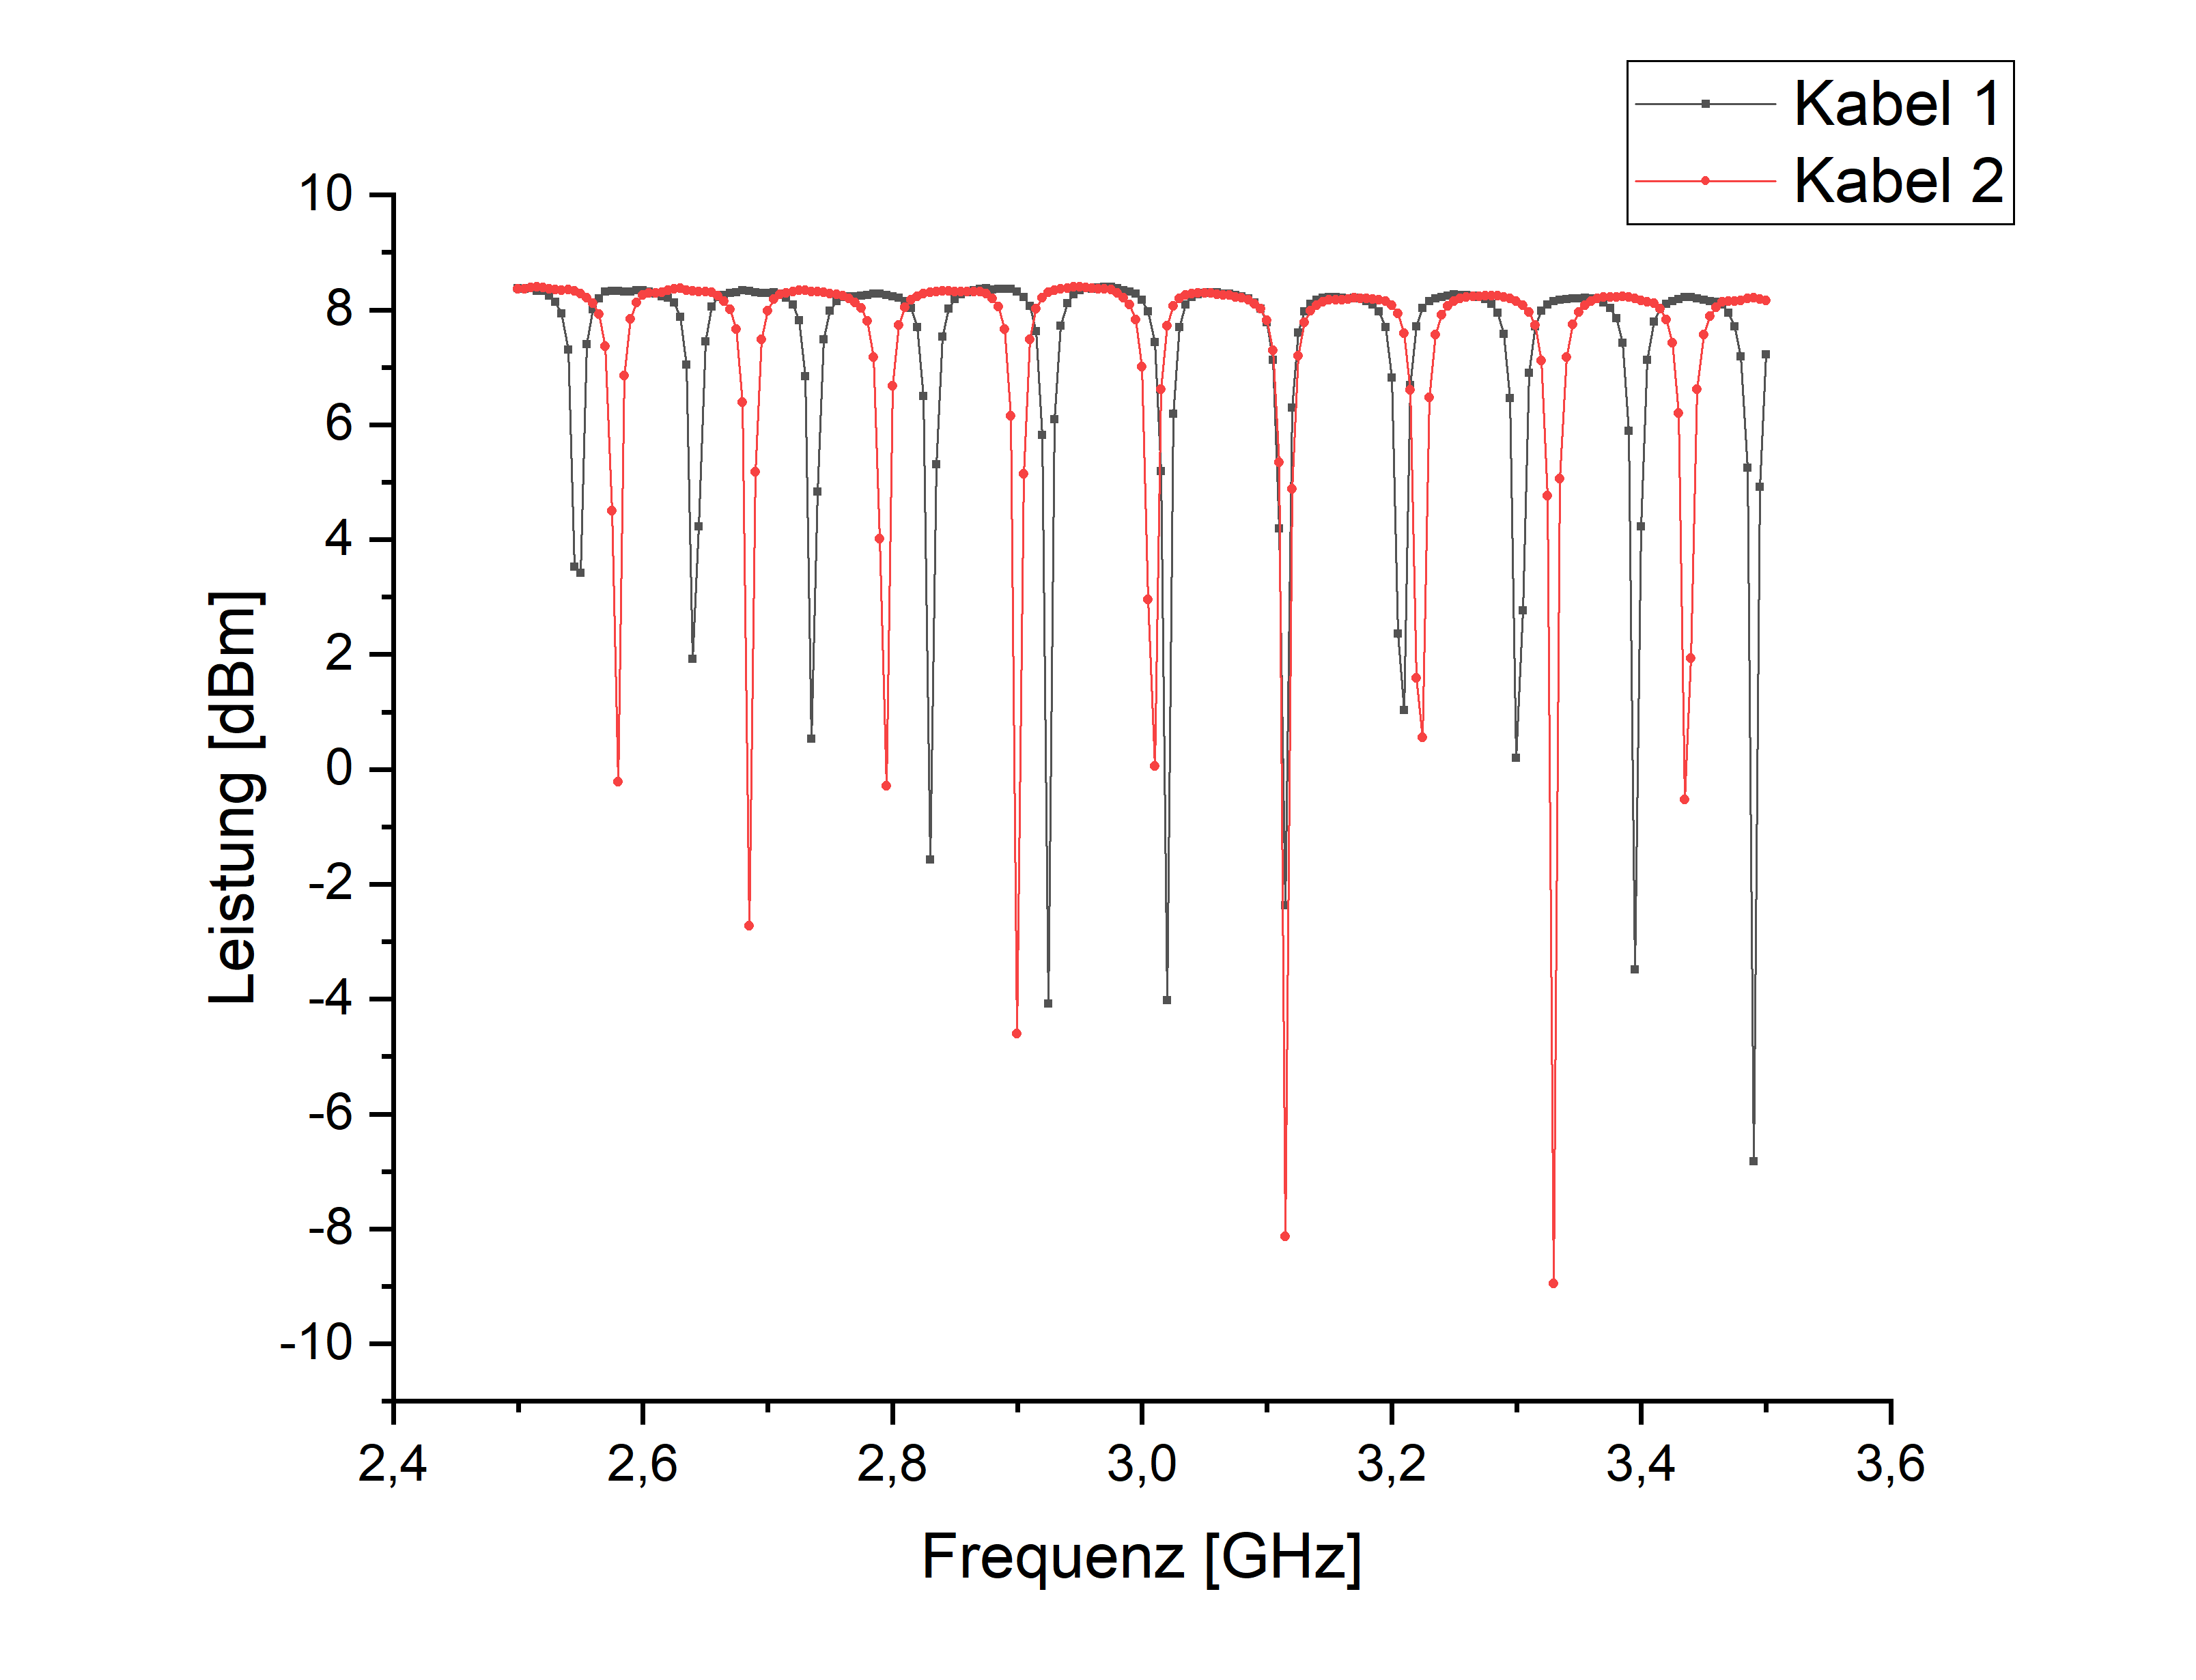
\includegraphics[scale=0.8]{anderes_Kabel.png}
	\caption{Leistung in Abhängigkeit der Frequenz für offenes Kabelende für Kabel 1 und 2. Deutlich erkennbar sind die unterschiedlichen Abstände zwischen den Resonanzen.}
	\label{anderes}
\end{figure}

Auf die gleiche Weise wie oben wurde anschließend der mittlere Abstand zweier benachbarter Resonanzen bestimmt, hierfür ergibt sich ein Wert von $\SI{0,106\pm0,002}{GHz}$. Dieser ist signifikant größer als der von Kabel 1.